% Integers 1 to 60. Multiples of 2, 3 and 5 are crossed; 2, 3 and 5 themselves are ringed.
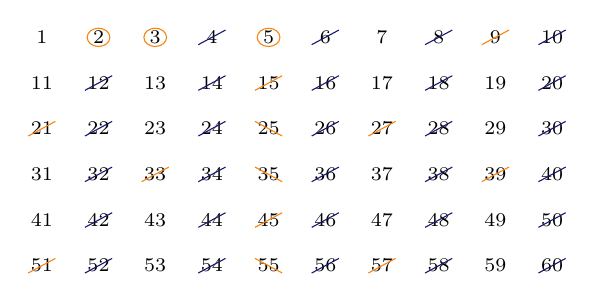
\begin{tikzpicture}[x=0.72cm,y=0.58cm,every node/.style={font=\scriptsize,inner sep=0pt}]
  \foreach \n in {1,...,60} {
    \pgfmathtruncatemacro{\col}{mod(\n-1,10)}
    \pgfmathtruncatemacro{\row}{int((\n-1)/10)}
    \pgfmathtruncatemacro{\mtwo}{mod(\n,2)}
    \pgfmathtruncatemacro{\mthree}{mod(\n,3)}
    \pgfmathtruncatemacro{\mfive}{mod(\n,5)}
    \node at (\col,-\row) {\n};
    \ifnum\n=2
      \draw[BurntOrange] (\col,-\row) circle (0.20);
    \else\ifnum\n=3
      \draw[BurntOrange] (\col,-\row) circle (0.20);
    \else\ifnum\n=5
      \draw[BurntOrange] (\col,-\row) circle (0.20);
    \else
      \ifnum\mtwo=0
        \draw[MidnightBlue] ({\col-0.24},{-\row-0.16})--({\col+0.24},{-\row+0.16});
      \else
        \ifnum\mthree=0
          \draw[BurntOrange] ({\col-0.24},{-\row-0.16})--({\col+0.24},{-\row+0.16});
        \else\ifnum\mfive=0
          \draw[BurntOrange] ({\col-0.24},{-\row+0.16})--({\col+0.24},{-\row-0.16});
        \fi\fi
      \fi
    \fi\fi\fi
  }
\end{tikzpicture}
